\outlineSubframe{Backtracking}
\begin{frame}{Allgemeines}{Eigenschaften}
    \begin{itemize}
        \item Grundlegende Algorithmenstrategie
        \item Findet theoretisch:
        \begin{itemize}
        \item alle Lösungen für ein gegebenes Problem...
        \item ...in einer endlichen Zeit
        \end{itemize}
        \item Nutzt das \textbf{trial and error} Prinzip
    \end{itemize}
\end{frame}

\begin{frame}{Methodik}
    \begin{itemize}
        \item Sind rekursiv implementiert
        \item Es werden inkrementell Teillösungen "`ausprobiert"'
        \item Wird eine Teillösung als ungeeignet erkannt, wird diese verworfen
        \item Implikationen daraus:
        \begin{itemize}
            \item Problem muss ein Kriterium für Nicht-Erfüllbarkeit liefern
            \item Oder anders: Die Lösung muss bestimmte Bedingungen erfüllen
            \item Man spricht in der Regel von \textbf{Constraint-Satisfaction-Problems}
        \end{itemize}
        \item Visualisieren lässt sich das z.B. als Entscheidungsbaum
    \end{itemize}
\end{frame}

\begin{frame}{Entscheidungsbaum}{Backtracking Algorithmen}
    \begin{figure}
    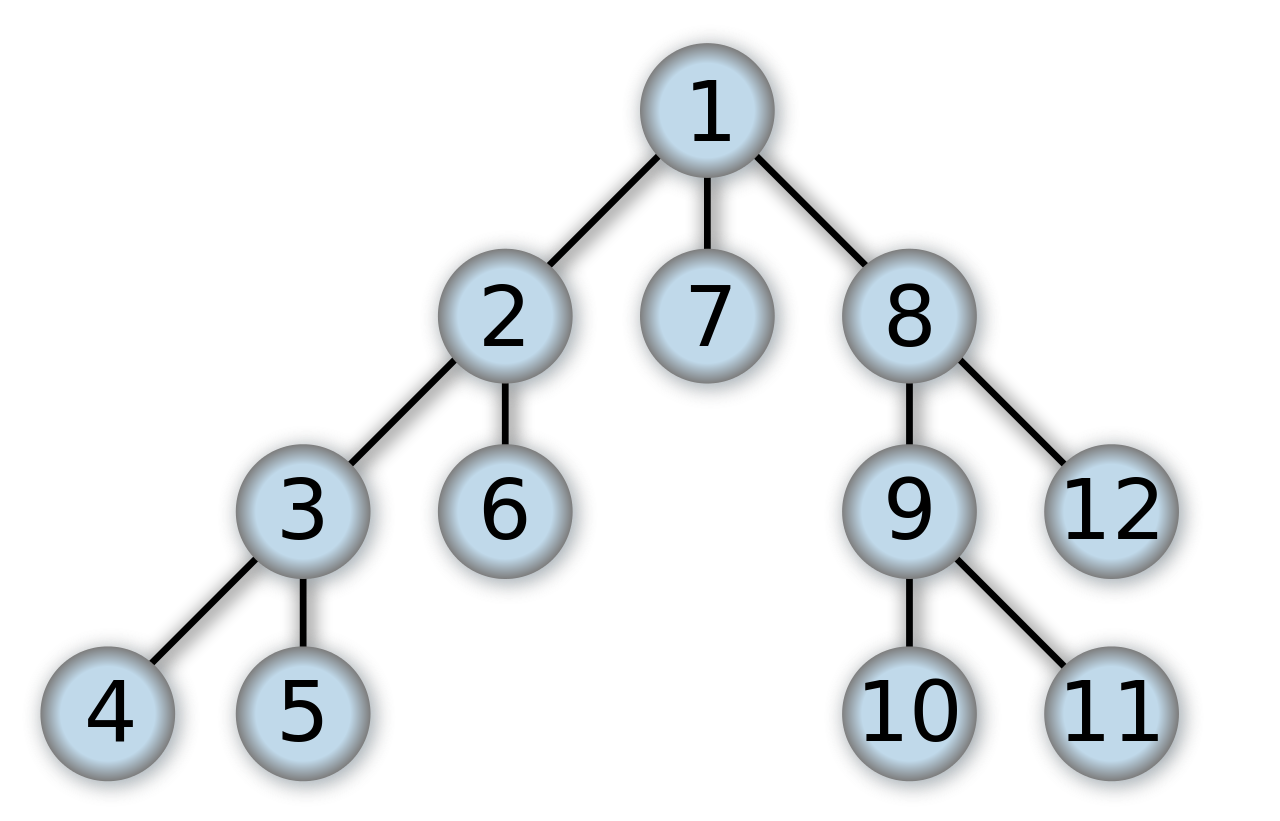
\includegraphics[height=5cm]{graph/backtracking_tree}
    \caption*{Quelle: \cite{wiki:backtr}}
    \end{figure}
\end{frame}

\begin{frame}{Vor- und Nachteile}
    \begin{itemize}
        \item Es werden alle (sinnvollen) Lösungen ausprobiert
        \item Umgekehrt kann definitiv ausgesagt werden, dass keine Lösung existiert, wenn Sie nicht über Backtracking gefunden werden kann
        \item Jedoch sehr ineffizient
        \begin{itemize}
            \item Komplexität im Worst Case ist $O(z^n)$ (Wobei $z$ der Verzweigungsgrad ist)
            \item Somit ergibt sich für alle $z>1$ eine exponentielle Laufzeit
            \item Daher eher für Probleme mit kleinem Lösungsbaum geeignet
        \end{itemize}
    \end{itemize}
\end{frame}

\begin{frame}[allowframebreaks]{Anwendungen}{Von Backtracking (Vgl. \cite{wiki:backtracking})}
    \begin{itemize}
        \item \textbf{Damenproblem}
        \begin{itemize}
            \item Auf einem $n\times n$ Schachfeld sollen $n$ Damen so platziert werden, dass sie sich nicht gegenseitig schlagen können
        \end{itemize}
        \item \textbf{Springerproblem}
        \begin{itemize}
            \item Auf einem $M\times N$ Schachfeld soll ein Springer einen Weg finden, durch den jedes Feld \textbf{genau einmal} besucht wird.
        \end{itemize}
        \item \textbf{Sudoku}
        \item \textbf{Färbeproblem}
        \begin{itemize}
            \item Eine Landkarte mit $B$ Ländern soll mit $N$ verschiedenen Farben eingefärbt werden
            \item Gesucht wird eine Einfärbung, bei der angrenzende Länder immer verschiedene Farben haben
        \end{itemize}
        \item \textbf{Wegsuche in Graphen}
        \begin{itemize}
            \item Hierzu gehört zum Beispiel auch das finden eines Weges in einem Labyrinth
        \end{itemize}
        \item Viele Backtracking Probleme sind \textbf{NP-vollständig}
    \end{itemize}
\end{frame}